\subsection*{b. Obtener una relación de los productos que pertenecen a la categoría Technology con precio mayor de \$400 y menor de \$850, pero que no hayan sido solicitados en ninguna orden.}

Primero seleccionamos los productos de la categoría \textit{Technology} cuyo precio sea mayor a 400 y menor a 850. Después obtenemos los id de los productos que sí han sido solicitados en alguna orden; restamos estos id a los de los productos seleccionados, por lo que quedan únicamente los productos que no han sido solicitados. Realizamos un join natural con la tabla \textit{products} para recuperar toda la información de los productos

Expresión:
\begin{equation}
\left( \pi_{productid}\left(\sigma_{category = \text{'Technology'} \, \wedge \, price > 400 \, \wedge \, price < 850}(products)\right) - \pi_{productid}(orders) \right) \bowtie products
\end{equation}

Resultados obtenidos:

\begin{figure}[h!]
\centering
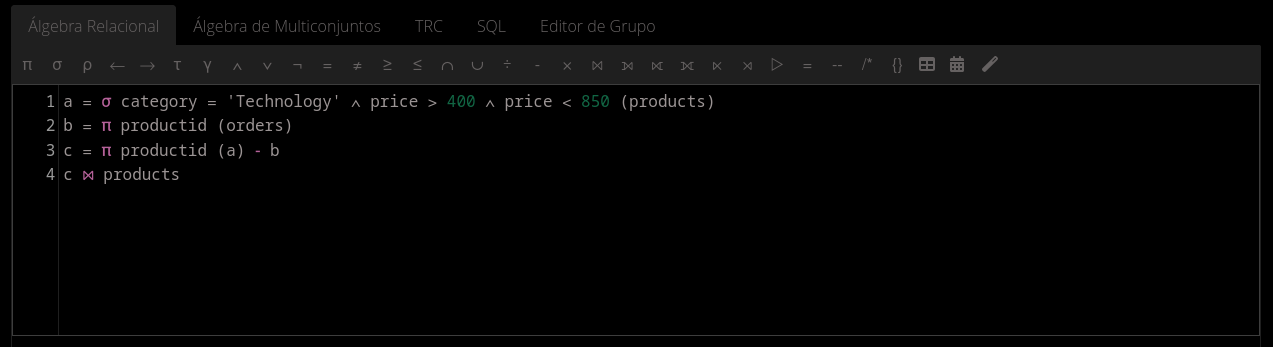
\includegraphics[width=0.8\textwidth]{imagenes/2b(1).png}
\caption{Consulta}
\end{figure}

\begin{figure}[h!]
\centering
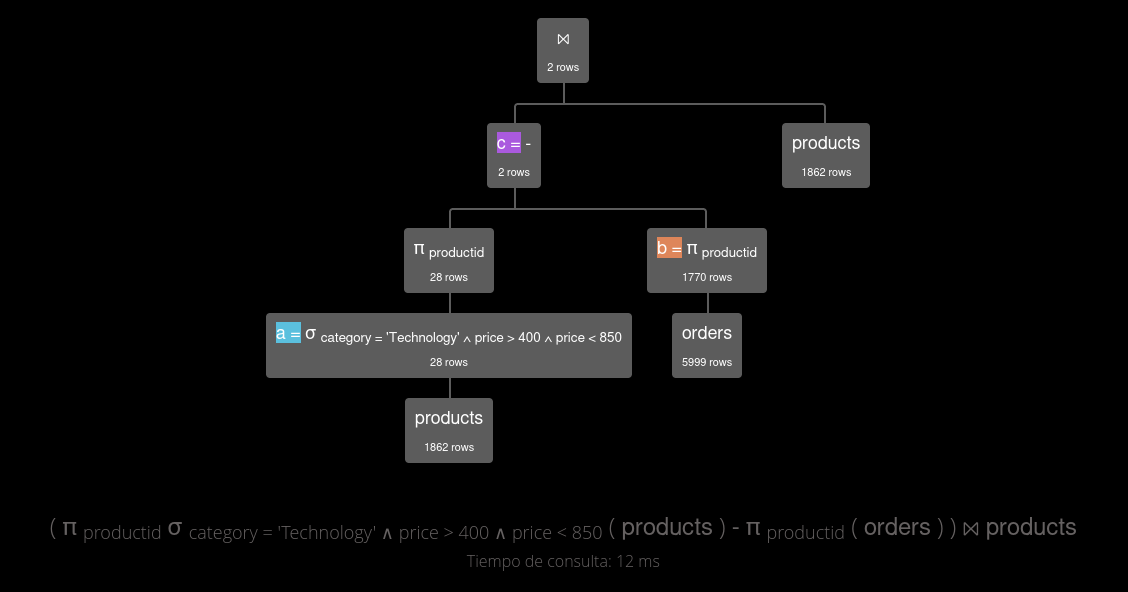
\includegraphics[width=0.8\textwidth]{imagenes/2b(2).png}
\caption{Árbol de consulta.}
\end{figure}

\begin{figure}[h!]
\centering
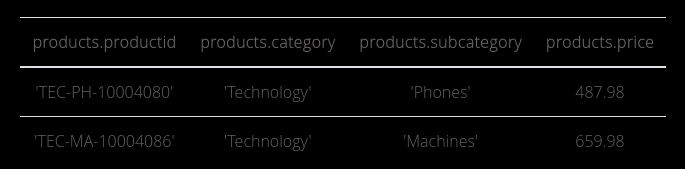
\includegraphics[width=0.6\textwidth]{imagenes/2b(3).png}
\caption{Resultado de consulta.}
\end{figure}